\section{Background and Related Work}

\subsection{Deep Research Agents}
% Deep research agents address long-horizon, open-ended information-seeking tasks by iteratively reasoning and interacting with external tools such as search engines and web browsers. 
Given an input question, deep research agents operate in a multi-step loop that alternates between reasoning to generate an action, executing the tool call, and incorporating the response into its context, until producing a final answer~\cite{zhang2025agentorchestra,huang2025deep}.


\begin{figure}
\centering
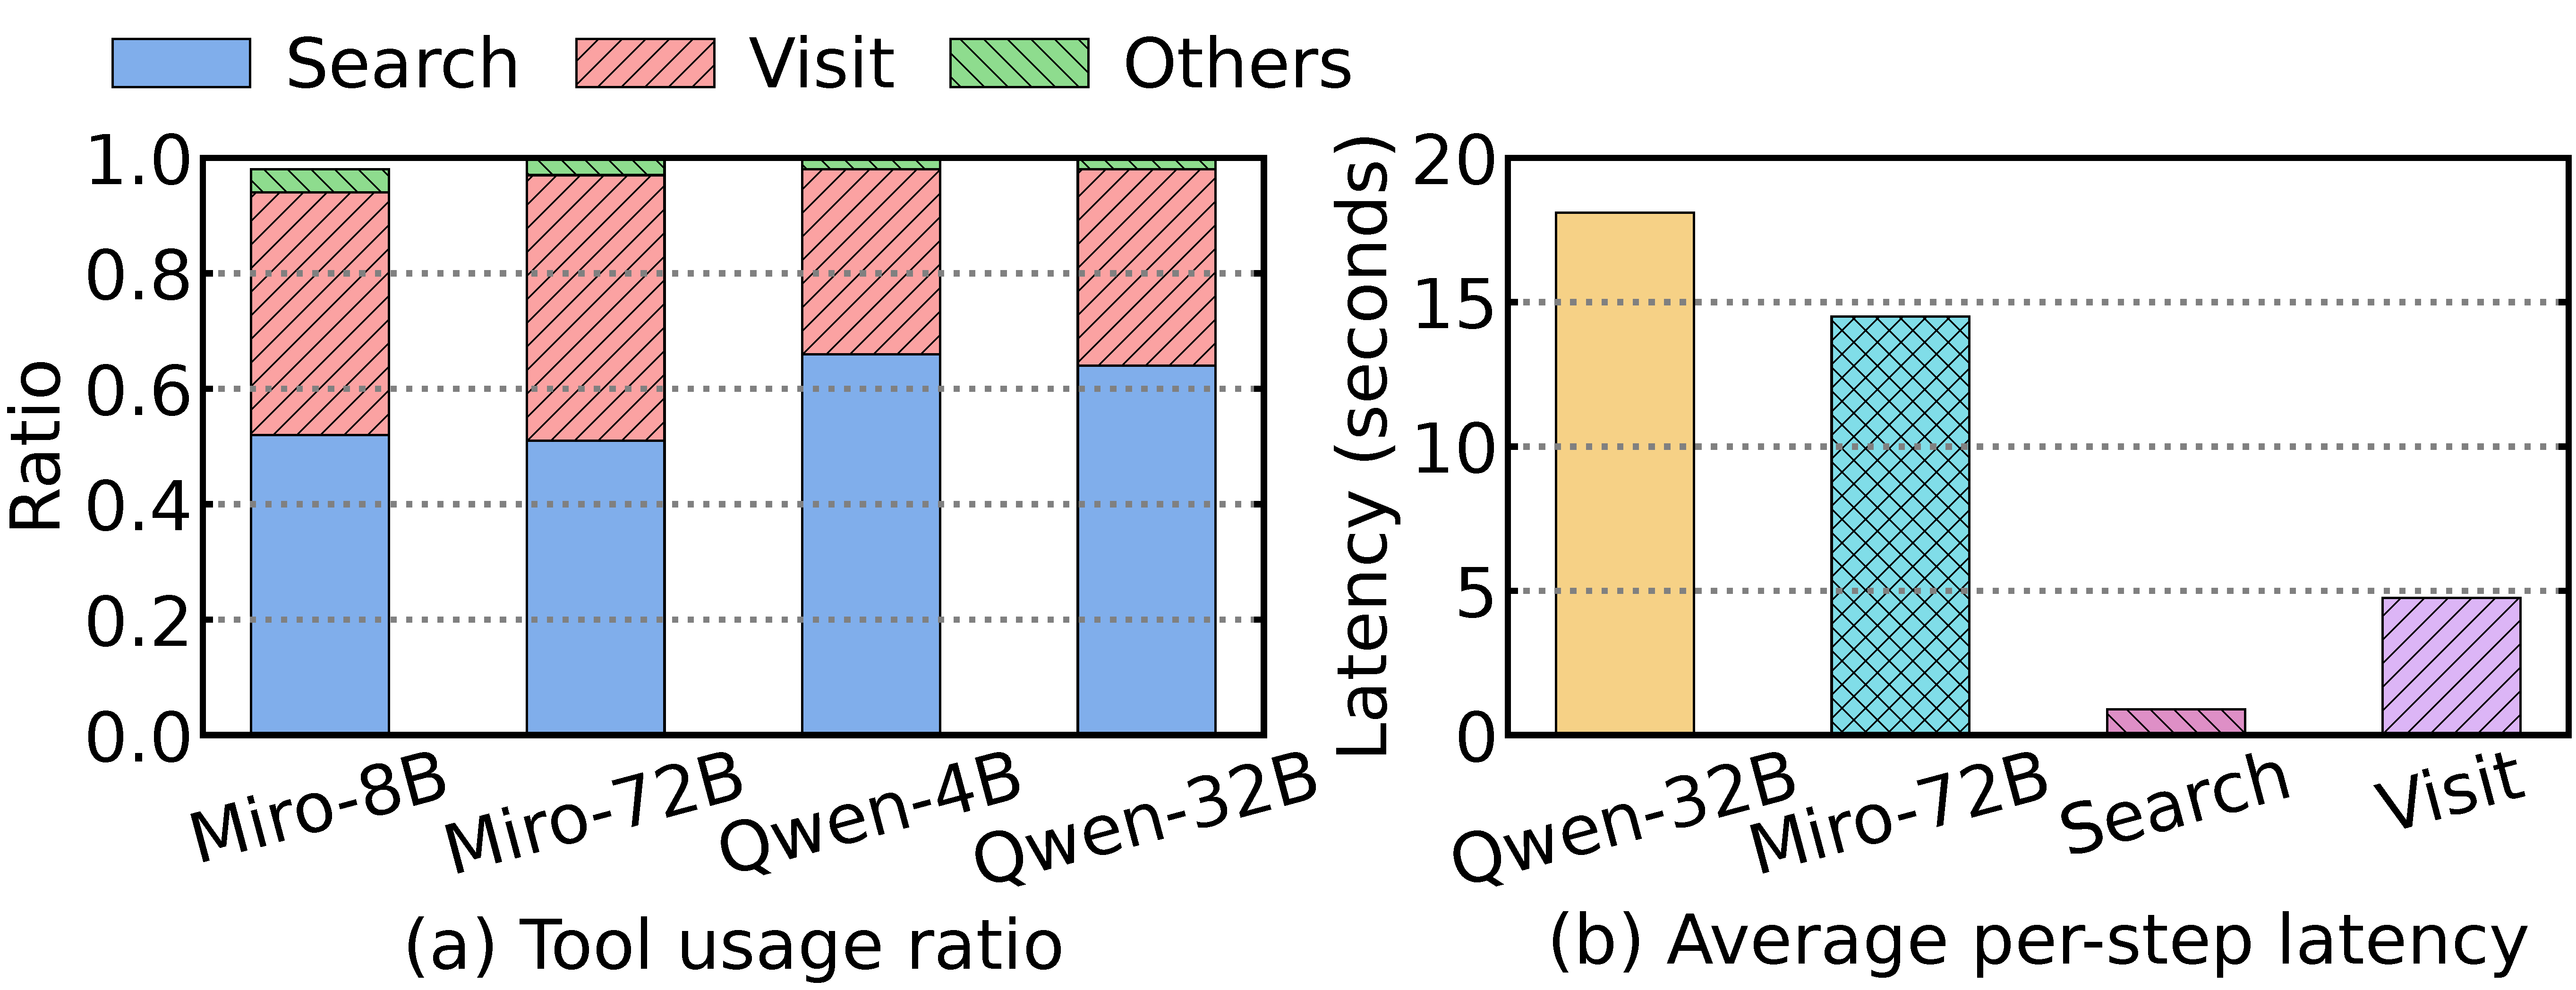
\includegraphics[width=\linewidth]{figs/draw_basics.pdf}
\caption{
Deep research inference characteristics using different models. ``Miro'' denotes ``MiroThinker'' while 
``Qwen'' denotes ``Qwen-3''.     
(a) Tool usage ratio on the GAIA benchmark\footnotemark. (b) Time breakdown per step on model reasoning and tool execution. Model reasoning accounts for a significant fraction of the total latency.}
\label{fig:action_ratio}
\end{figure}

\footnotetext{Unless otherwise specified, all micro-level analyses are conducted on the GAIA benchmark; consistent trends are observed across other benchmarks.}

% Most deep research agents rely on two core actions in their workflows: \textit{Search} and \textit{Visit}. 
% The \textit{Search} action formulates a query to retrieve a list of candidate webpages, each 
% accompanied by a brief snippet. 
% The \textit{Visit} action then selects a specific URL and provides a concise instruction 
% specifying what information to extract from the page. 
% To execute these actions, \textit{Search} directly interacts with a search engine, 
% whereas \textit{Visit} accesses the selected webpage and typically invokes an LLM to summarize 
% task-relevant content according to the instruction. 
% This design helps filter out irrelevant information and limits unnecessary context growth in the agent. 
% Figure~\ref{fig:action_ratio}(a) reports 
% the relative frequency of these actions when running tasks on the GAIA benchmark.  
% The results demonstrate that they are used at comparable rates, with \textit{Search} occurring slightly 
% more often due to query reformulation when retrieved results are unsatisfactory.
% Other tool calls (e.g., code execution) account for only a small fraction of steps.

Most deep research agents rely on two core actions: Search and Visit.
Search consists of a query used to retrieve candidate webpages with brief snippets, while Visit selects a URL and specifies an instruction for extracting relevant information.
During execution,
Search directly queries a search engine, whereas Visit accesses the webpage and typically invokes an LLM to summarize task-relevant content according to the instruction\cite{nakano2021webgpt, zhou2023webarena}.
This design filters irrelevant information and limits unnecessary context growth.
Figure~\ref{fig:action_ratio}(a) shows that these actions occur at comparable frequencies, with Search used slightly more often due to query reformulation when results are unsatisfactory.
Other tool calls (e.g., code execution) constitute only a small fraction of steps.


% Despite strong problem-solving capabilities, deep research agents often incur high latency due to the multi-step nature of their reasoning and tool-use workflows. We measure the per-step time breakdown by running the agent on the A100 GPU and show the results Figure~\ref{fig:action_ratio}(b). Model reasoning constitutes a significant portion of the total latency, while tool execution introduces additional, though smaller, delays. When accumulated over many iterations, these costs lead to long end-to-end response times, hindering user experience and practical deployment. 

Despite strong problem-solving performance, deep research agents often incur high latency due to their multi-step reasoning and tool-use workflows.
Figure~\ref{fig:action_ratio}(b) reports the per-step time breakdown measured on the A100 GPU.
Model reasoning dominates total latency, while tool execution introduces additional, though smaller, overheads.
Accumulated over many iterations, these costs lead to long end-to-end response times, limiting usability and deployment.

\subsection{Agent Optimization}

% Stronger backbone models and richer interactions with external tools improve agent performance on challenging tasks~\cite{yao2022react}.
% However, these gains often come at the cost of time efficiency, as longer reasoning traces and more frequent tool interactions lead to increased latency. 
% Recent studies observe that not all agent steps are equally challenging~\cite{zhang2023ecoassistant,saha2024system}. 
% This insight motivates optimization techniques that offload simpler steps to lightweight models while reserving more complex reasoning for stronger models, thereby balancing performance and efficiency.

Stronger backbone models and richer tool interactions improve agent performance on challenging tasks~\cite{shang2025rstar2}, but often reduce time efficiency due to longer reasoning traces and more frequent tool use.
Recent work observes that agent steps vary in difficulty~\cite{zhang2023ecoassistant,saha2024system}, motivating approaches that delegate simpler steps to lightweight models while reserving complex reasoning for stronger models.

% In this context, speculate--verify paradigms have emerged as a promising direction for reducing agent latency~\cite{ye2025speculative,guan2025dynamic,hua2024interactive,wang2025accelerating}. 
% Dynamic Speculative Planning~\cite{guan2025dynamic} introduces a lightweight speculator (e.g., a small reasoning model) to draft an action and obtain its result, while a stronger base model concurrently performs full reasoning. 
% The speculative action is verified against the base model action using criteria such as minimum edit distance, and the speculative tool call response is reused when they agree, reducing overall latency. 
% SPAgent~\cite{huang2025reducing} skips explicit reasoning in early stages to generate actions, and transitions to a speculate--verify phase later to preserve the agent performance. 

Speculate--verify paradigms have emerged as an effective strategy to reduce agent latency~\cite{ye2025speculative,guan2025dynamic,hua2024interactive,wang2025accelerating}.
Dynamic Speculative Planning~\cite{guan2025dynamic} employs a small reasoning model to draft an action and obtain its result while a stronger model performs full reasoning; the speculative action is verified against the base model's action using criteria such as minimum edit distance, and its tool response is reused upon agreement.
SPAgent~\cite{huang2025reducing} skips explicit reasoning in early stages and transitions to a speculate--verify phase later to maintain performance.

At a finer granularity, speculative decoding~\cite{leviathan2023fast} accelerates LLM inference at the token level by predicting future tokens with a smaller model and verifying them with a larger model. 
This approach is complementary to agent-level speculation and can be combined with it to further improve efficiency. 
SpecReason~\cite{pan2025specreason} reduces reasoning overhead by dynamically offloading simpler reasoning steps to a smaller model; however, it is not designed for agent-based settings with iterative tool use.

% At finer granularity, speculative decoding~\cite{xia2024unlocking} accelerates token-level inference by predicting future tokens with a smaller model and verifying them with a larger one.
% This technique is complementary to agent-level speculation.
% SpecReason~\cite{pan2025specreason} dynamically offloads simpler reasoning steps to a smaller model, but is not designed for agent settings with iterative tool use.


\subsection{Dual-Process Theory in LLMs}
% Dual-process theory~\cite{chaiken1999dual} from cognitive science distinguishes between two modes of decision making: System~1, which is fast and intuitive, and System~2, which is slower and supports deliberate reasoning. 
% This framework has recently been adopted to interpret and guide reasoning behaviors in LLMs. 

% The System-1.x Planner~\cite{saha2024system} proposes a controllable planning framework that decomposes tasks into simpler and more complex sub-steps, assigning System~1 strategies to the former and System~2 strategies to the latter to improve efficiency. 
% However, this approach is limited to specific planning settings and requires extensive training. 
% How to systematically leverage dual-process principles in LLM-based agents with iterative tool use, such as deep research agents, remains largely unexplored.

Dual-process theory~\cite{chaiken1999dual} from cognitive science distinguishes between System~1, which is fast and intuitive, and System~2, which supports slower, deliberate reasoning.
This framework has recently been applied to interpret and guide LLM reasoning.
The System-1.x Planner~\cite{saha2024system} decomposes tasks into simpler and more complex sub-steps, assigning System~1 strategies to the former and System~2 strategies to the latter to improve efficiency.
However, it targets specific planning settings and requires extensive training.
How to systematically leverage dual-process principles in LLM-based agents with tool use, such as deep research agents, remains largely unexplored.
% Systematic application of dual-process principles to LLM-based agents with iterative tool use, such as deep research agents, remains largely unexplored.


% A growing body of work has explored methods to improve the performance of LLM-based agents on complex tasks. 
% Chain-of-thought prompting~\cite{wei2022chain} encourages LLMs to generate explicit step-by-step reasoning for each action. Subsequent approaches, such as ReAct~\cite{yao2022react}, further interleave reasoning traces with actions to better guide decision-making, while Reflexion~\cite{shinn2023reflexion} enables agents to self-reflect on past mistakes and adjust future behavior. 
% Overall, stronger backbone models and richer interactions with external tools have been shown to improve agent performance on challenging tasks.

% In LLMs, System 2 behavior is commonly associated with explicit reasoning traces that introduce intermediate structure, reduce uncertainty, and guide complex decisions, while System 1 behavior corresponds to direct generation driven by strong parametric priors. Importantly, whether explicit reasoning is beneficial depends on the nature of the task: for decisions with high ambiguity or weak local cues, reasoning can substantially improve reliability, whereas for decisions grounded in concrete context, reasoning may offer limited marginal benefit.

% We argue that this distinction naturally extends to action generation in deep research agents. Different actions impose different cognitive demands: some require deliberation to resolve underspecified goals, while others involve relatively direct operations on observed information. Recognizing and exploiting this heterogeneity provides a useful lens for understanding why uniform speculation strategies are suboptimal, and it motivates our approach to allocating inference resources asymmetrically across action types.